\documentclass{beamer}
\usepackage[utf8]{inputenc}
\usepackage{listings}
\usepackage{booktabs}
\usepackage{bm}
\usepackage{enumitem}
\usepackage[export]{adjustbox}
\usepackage{svg}

\usetheme{Madrid}
\definecolor{mlpblue}{rgb}{0.1, 0.14, 0.24}

\useoutertheme{infolines} % Alternatively: miniframes, infolines, split
\useinnertheme{circles}
\usecolortheme[named=mlpblue]{structure}

\lstset{basicstyle=\footnotesize\ttfamily,breaklines=true}

%------------------------------------------------------------
%This block of code defines the information to appear in the
%Title page
\title[G-Transformation Invaraiance]{Neural Networks for Learning Counterfactual G-Invariances from Single Environments}

\subtitle{``Fixing the Image Rotation Problem''}

\author[COM 314] % optional
{J.~Setpal} 

\date{\today}

\titlegraphic{
\includegraphics[width=7cm]{../shared/logo-long.pdf}}

%End of title page configuration block
%------------------------------------------------------------

%The next block of commands puts the table of contents at the 
%beginning of each section and highlights the current section:

\AtBeginSection[]
{
  \begin{frame}
    \frametitle{Outline}
    \tableofcontents[currentsection]
  \end{frame}
}
% ------------------------------------------------------------


\begin{document}

%The next statement creates the title page.
\frame{\titlepage}

\begin{frame}{Neural Networks Aren't Rotationally Robust.}
	\textbf{Q}${}_1$: Do you think that a CNN trained on a distribution of the left image \textit{should} classify the right image as the same class for each of these pairs?
	\vspace{-.9em}
	\begin{center}
		
\includegraphics[width=\textwidth]{img/rot.png}
	\end{center} 
	\pause
	\vspace{-1em}
	\textbf{A}${}_1$: Definitely! \pause \newline \\
	\textbf{Q}${}_2$: In practice, does this actually happen? \pause \\
	\textbf{A}${}_2$: Nope -- all these images were misclassified. \pause \newline \\
	\textbf{Q}${}_3$: How can we fix this? \pause \\
	\textbf{A}${}_3$: Data Augmentation (boring)\pause, \textbf{G-Invariant Transformations} (fun)!
\end{frame}

\begin{frame}{Images as Transformations}
	We can visualize the image rotations as \underline{affine matrix transformations}:
	\begin{gather}
		G_{rot} \equiv \{T^{0^\circ}, T^{90^\circ}, T^{180^\circ}, T^{270^\circ}\} \\
		x_{new} = T x_{orig}; T \in G_{rot}
	\end{gather}
	\vspace{-2em}
	\begin{center}
		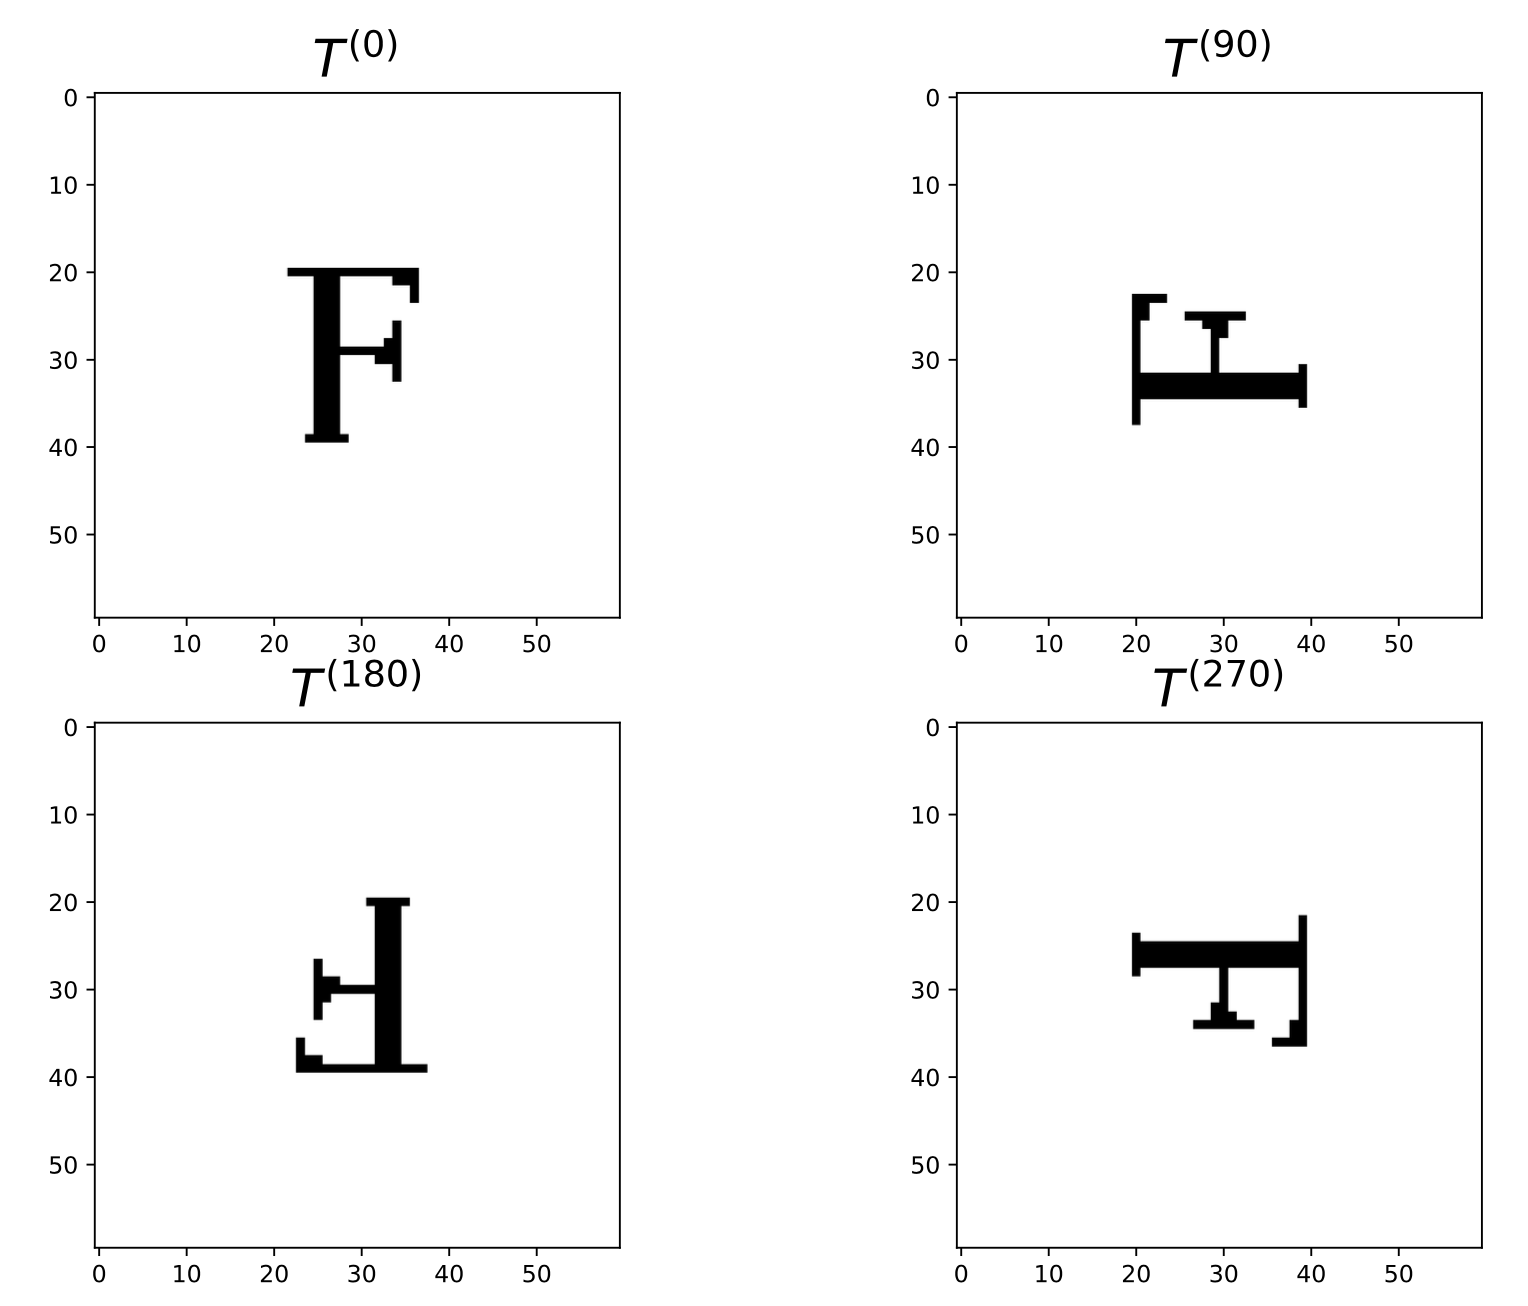
\includegraphics[width=0.5\textwidth]{img/f_rots.png}
	\end{center}
\end{frame}

\begin{frame}{Mathematical Formulation}
	Defining the transformations as a \textbf{group} gives us \textit{guarantees} we can exploit to ensure \textbf{invariance} to those transformations. \pause \newline \\

	Formally, we create an embedding layer to achieve the following:
	\begin{gather}
		\sigma(w^Tx + b) \stackrel{def}{=} \sigma(w^T \bm{T} x + b); \bm{T} \in G_{rot}
	\end{gather} \pause
	This is only possible if we can find a transformation $\bar{T}$ such that:
	\begin{gather}
		\bar{T}(\bm{T} x) = \bar{T} x;~\text{same as }
		\bar{T}x_{new} = \bar{T} x_{orig}; 
	\end{gather} \pause
	\textbf{Lemma:} We can find $\bar{T}$ using the \textit{Reynold's Operator}.
	\begin{gather}
		\bar{T} = \frac{1}{|G|}\sum_{g \in G}g
	\end{gather} \pause
	Finally, we construct our group invariant layer:
	\begin{gather}
		h_{inv} = \sigma(w^T\bar{T}x + b)
	\end{gather}
\end{frame}

\begin{frame}{Let's Demonstrate!}
	Here's what the final architecture looks like:
	\begin{center}
		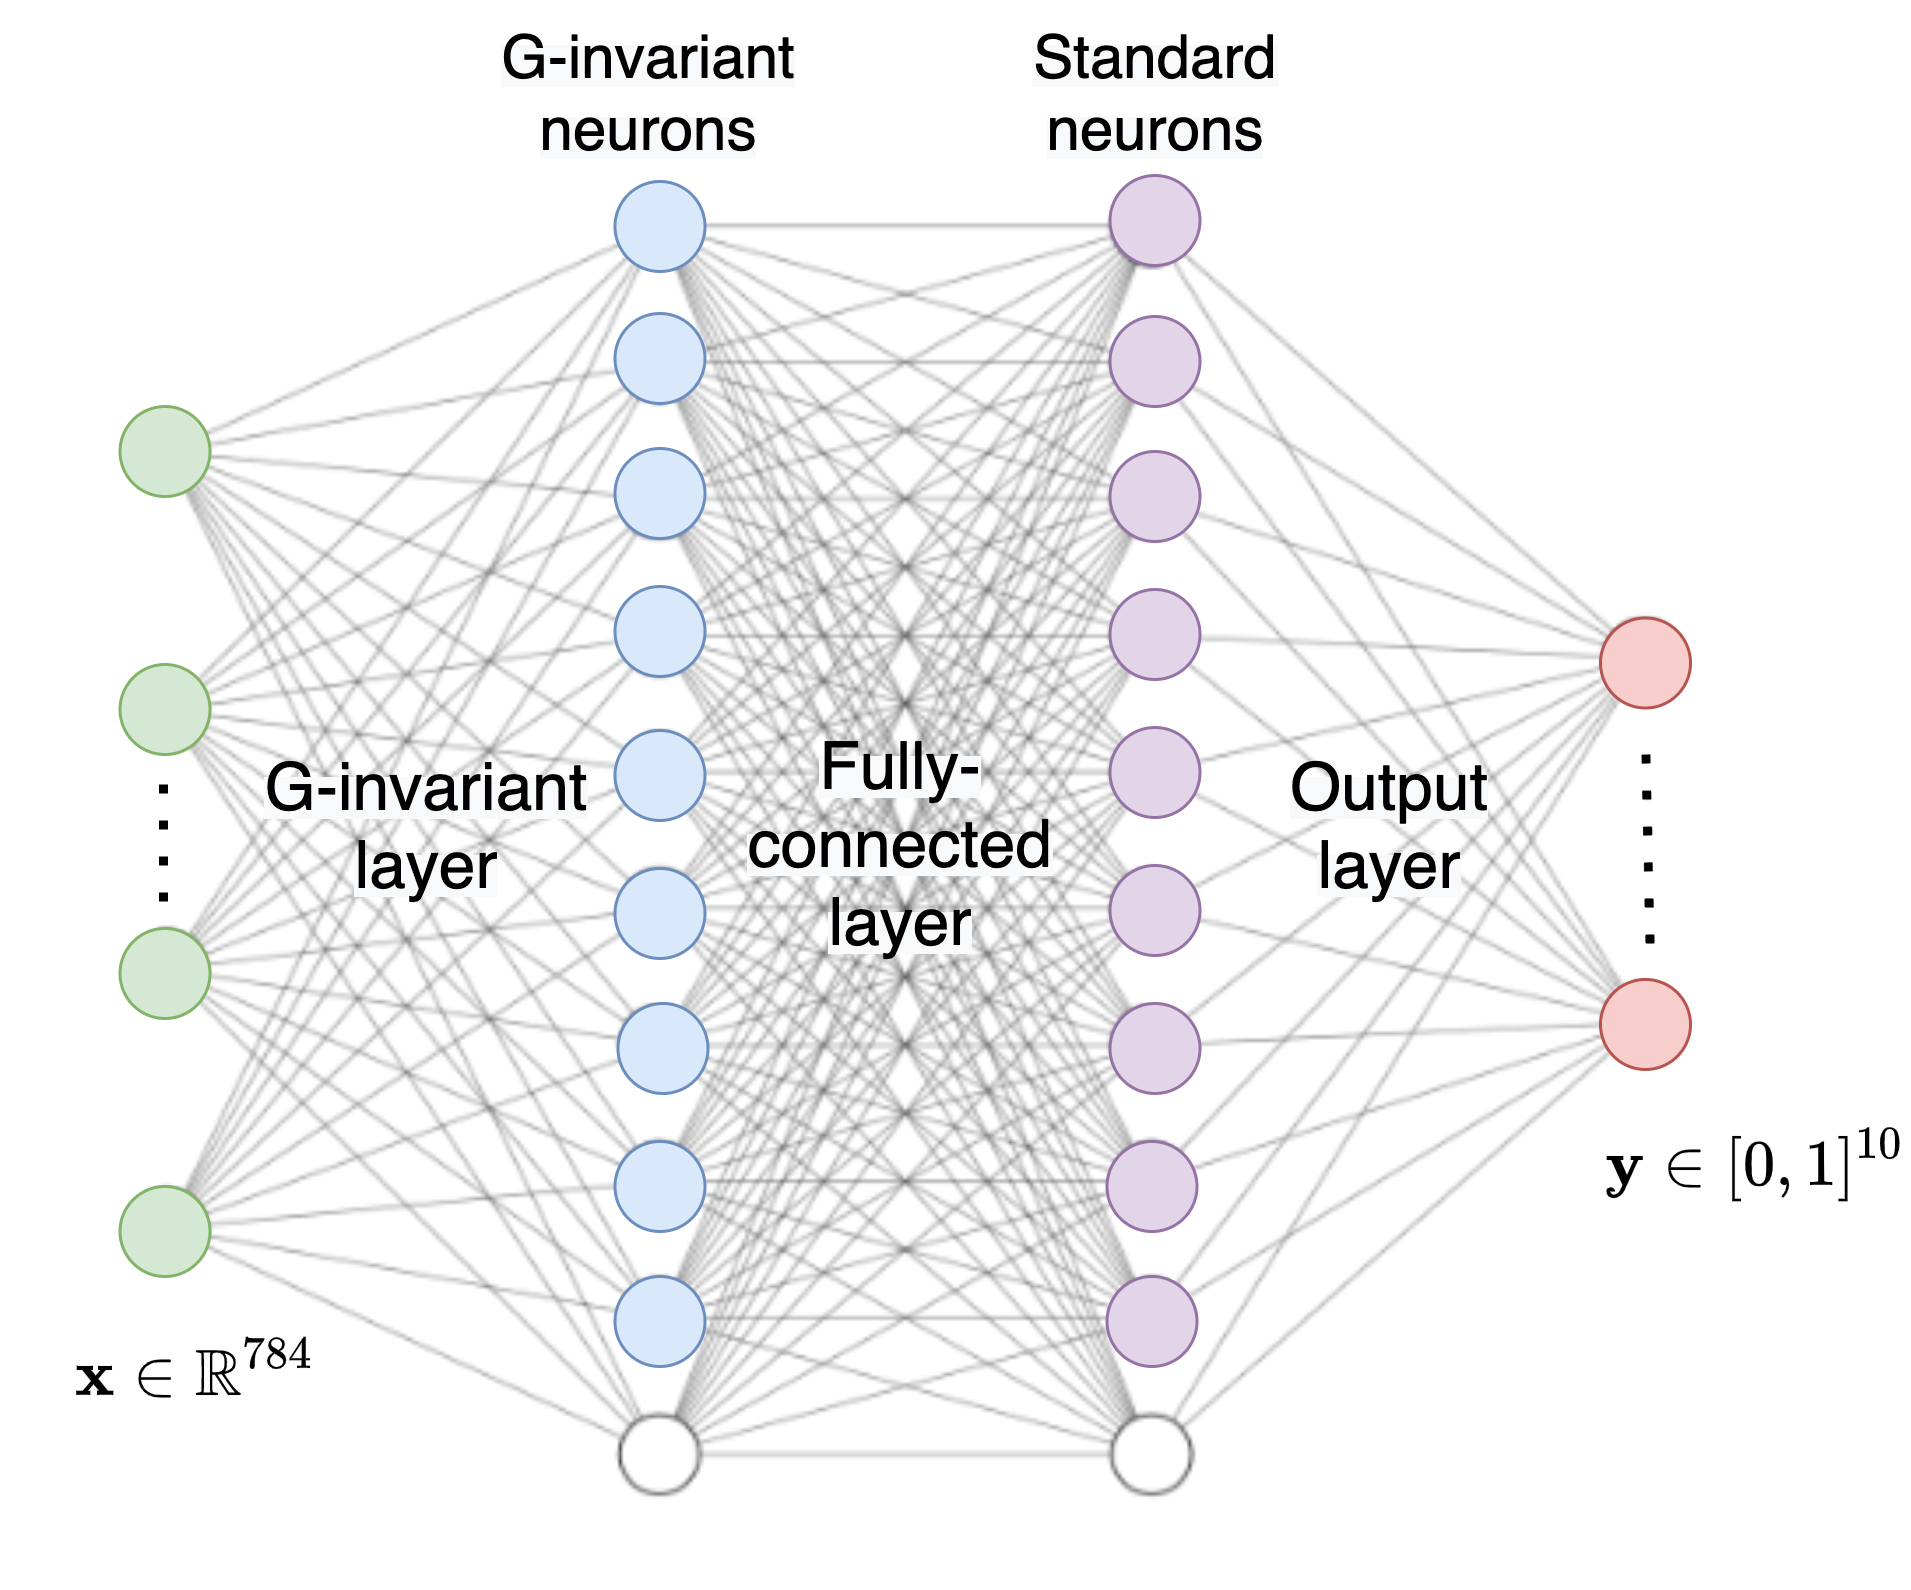
\includegraphics[width=.7\textwidth]{img/mlp.png}
	\end{center}
\end{frame}

\begin{frame}{Thank you!}
	\begin{center}
		Hopefully, this was cool!
	\end{center}
	\begin{align*}
		\textbf{\small Paper:}&~\texttt{\small\url{https://arxiv.org/abs/2104.10105/}} \\
		\textbf{\small Slides:}&~\texttt{\small\url{https://cs.purdue.edu/homes/jsetpal/slides/gti.pdf}} \\
		\textbf{\small Notebook:}&~\texttt{\small\url{https://cs.purdue.edu/homes/jsetpal/nb/gti.ipynb}} \\
		\textbf{\small Presentation:}&~\texttt{\small\url{https://www.youtube.com/watch?v=znJsaCGiu10}}
	\end{align*}
\end{frame}

\end{document}
